\documentclass[letterpaper,twoside,12pt]{article}
\usepackage[T1]{fontenc}
\usepackage{textcomp}
%\usepackage[dvips]{graphicx}
\usepackage{graphicx}
\usepackage{epstopdf}
\usepackage[margin=0.8in]{geometry}
\usepackage{caption}
\usepackage{amsmath}
\usepackage{amssymb}
\usepackage[T1]{fontenc}
\usepackage{natbib}
\usepackage{authblk}
%\usepackage{fancyvrb}
%\usepackage{lmodern}
%\usepackage{url}
%\usepackage{times}
\usepackage{textcomp}
%\usepackage{parskip}
\bibliographystyle{agu08}

\newcommand{\ud}{\mathrm d}
\newcommand{\uj}{\mathrm{j}}
\newcommand{\bz}{\mathbf{z}}
\newcommand{\Real}{\mathrm{Re}}
\newcommand{\Imag}{\mathrm{Im}}
\newcommand{\dif}{\mathrm{d}}
\newcommand{\sigsig}{\sigma_1\sigma_2}
\newcommand{\varss}{\varsigma_1\varsigma_2}
\newcommand{\hvarss}{\hat{\varsigma}_1 \hat{\varsigma}_2}
\newcommand{\twodots}{\mathinner {\ldotp \ldotp}}
\newcommand{\midtilde}{\raisebox{0.5ex}{\texttildelow}}

\DeclareMathOperator\erf{erf}

\title{Comparison of Linear and Circular Products after PolConvert}

\author[1]{L. V. Benkevitch}
\affil[1]{\small MIT Haystack observatory, Westford, MA 01886, USA.}


\begin{document}

\maketitle

\begin{abstract}

The VGOS data are collected with the use of linearly polarized receivers. However, circular polarization has a number of benefits. The PolConvert software allows VGOS data conversion from linear to circular polarization. In this study we do a statistical comparison of the pseudo-Stokes data before and after the conversion in order to characterize the errors PolConvert introduces.

\end{abstract}


\tableofcontents


\section{Parameter Temporal Variations Before and After PolConvert}

Converting linear polarization of the source data to the circular polarization with the PolConvert software introduces changes into its properties. Here we consider the changes in multi-band delays (MBD), single-band delays (SBD), and signal-to-noise ratios (SNR) for the pseudo-Stokes polarization products, of which we only select the pseudo-Stokes $I$ parameters as functions of time, $t$. From the original, linearly polarized data set we read $I$, which we denote LinI($t$). PolConvert is applied to the original data set and generates another data set with circular polarization, from which we read $I$ parameters denoted as CirI($t$). Of course, the data are presented in the discrete, numerical format, so instead of the continuous time, $t$, integer indices are used, like $k=\overline{1..N}$, where $N$ is the number of data points in the sample.  The following Figures show temporal variations of the LinI[$k$] and CirI[$k$] parameters during the experiment before and after PolConvert, one graph for each baseline:  \\


\indent MBD variations in Fig.~\ref{mbd_lin_and_cir};  \\
\indent SBD variations in Fig.~\ref{sbd_lin_and_cir};  \\
\indent SNR variations in Fig.~\ref{snr_lin_and_cir}.  \\


One can see that most of the graphs after PolConvert, CirI[$k$], are significantly biased with respect to LinI[$k$]. The biases calculated as $\mathrm{LinI}[k] - \mathrm{CirI}[k]$ are plotted in the Figures below: \\

\indent MBD bias variations in Fig.~\ref{mbd_lin_cir_bias};  \\
\indent SBD bias variations in Fig.~\ref{sbd_lin_cir_bias};  \\
\indent SNR bias variations in Fig.~\ref{snr_lin_cir_bias}.  \\

However, removing the bias by subtracting the mean values of each curve makes the differences much less significant:

\begin{equation}
  \label{subtr_mean_lin}
  \mathrm{LinI}[k] = \mathrm{LinI}[k] - \mathrm{mean(LinI}[k])
\end{equation}

\begin{equation}
  \label{subtr_mean_cir}
  \mathrm{CirI}[k] = \mathrm{CirI}[k] - \mathrm{mean(CirI}[k])
\end{equation}

\noindent In order to compare the unbiased LinI[$k$] with CirI[$k$], the residual, res[$k$], is computed as their difference:

\begin{equation}
  \label{resid}
  \mathrm{res}[k] = \mathrm{LinI}[k] - \mathrm{CirI}[k] 
\end{equation}

\noindent The graphs of residuals with the means subtracted are shown in the following Figures: \\

\indent MBD residual variations in Fig.~\ref{mbd_lin_minus_cir};  \\
\indent SBD residual variations in Fig.~\ref{sbd_lin_minus_cir};  \\
\indent SNR residual variations in Fig.~\ref{snr_lin_minus_cir}.  \\

To assess the similarity of LinI[$k$] and CirI[$k$], the following parameters are computed: \\

\noindent - Pearson correlation coefficient $r_{corr}$; \\
\noindent - Root Mean Square Error, RMSE; \\

Since LinI[$k$] and CirI[$k$] already have their means subtracted, the correlation formula is simplified:

\begin{equation}
  \label{corr}
  r_{corr} = \frac{\sum \mathrm{LinI}[k] \cdot \mathrm{CirI}[k]}{\sqrt{\sum \mathrm{LinI}[k]^2 \cdot 
                   \mathrm{CirI}[k]^2}}
\end{equation}

The root mean square error, RMSE, in our case is actually the standard deviation of the residual, $\sigma$:

\begin{equation}
  \label{rmse}
  \mathrm{RMSE} = \sqrt{\frac{1}{N} \sum \mathrm{res}[k]^2}
\end{equation}

Lower RMSE indicates a better fit between the curves. However, RMSE is not an ``absolute'' indicator of the curves' proximity. The correlation coefficient, though, has its upper limit, unity, and if $r_{corr}$ is very close to unity, the curves are almost identical, save their constant bias. MBD and SNR demonstrate excellent correlations between LinI and CirI.


\section{Parameter residual Statistics Before and After PolConvert}

While in the previous Section MBD, SBD, and SNR pseudo-Stokes $I$ parameter data were treated as functions of time, here we do their statistical study. In order to estimate the errors introduced by PolConvert, histograms of the parameter residuals (after the mean subtraction, see Eqs.~\eqref{subtr_mean_lin} and \eqref{subtr_mean_cir}) are plotted. Below are the histograms for all of the baselines: \\

\indent MBD residual histogram for all of the baselines in Fig.~\ref{dmbd_distr};  \\
\indent SBD residual histogram for all of the baselines in Fig.~\ref{dsbd_distr};  \\
\indent SNR residual histogram for all of the baselines in Fig.~\ref{dsnr_distr}.  \\

Note that the means of the residuals are very close to zero (actually, down to the machine epsilon!). 

In order to evaluate the significance of the error we attempted to use the Pearson's chi-squared test comparing the histograms to the normal distributions:

\begin{equation}
  \label{normal_pdf}
  f(\mu,\sigma) =  \frac{1}{\sigma\sqrt{2\pi}} e^{-\frac{(x-\mu)^2}{2\sigma^2}}.
\end{equation}

Initially, all the histograms had 21 bins. The left-tail and right-tail bins with sparse data (frequencies less than 5) were grouped and the test used fewer number of bins (printed in each plot). The Pearson's $\chi^2$ test is based on comparing the observed data counts with the expected (theoretical) counts $E_i, i=\overline{1 \twodots N_b}$ obtained from the normal PDF~\eqref{normal_pdf} as $E_i = Np_i$. Here $p_i$ is the probability that a random value sampled from $N(\mu,\sigma)$ is within the $i$-th interval. The intervals are given in Tab.~\ref{quant_io}, where $i$ is one of the Output values. $\ldots\cdots\ldotp\ldotp$ The value of the test-statistic was calculated as

\begin{equation}
  \label{x2_calc}
  X^2 = \sum_{i=1}^{N_b} \frac{(B_i - E_i)^2}{E_i}.
\end{equation}


However, this method did not work: the residuals are grouped around their means substantially denser than the normal distributions with the same standard deviations. Calculated values of the histogram chi-squares are many times greater than the critical chi-square values for the p-values less than or equal to 0.05 (printed in each of the histogram plots). 

We have used another method. Since the residuals are mostly within $\pm \sigma$ (standard deviation), we  compute their proportion and compare it to the expected proportion under a normal distribution, which is about 68.27\%. The proportion is printed near each histogram. It is at the level of about 80\%, which is better the standard normal.

It is interesting to see which of the individual stations contribute to the errors. We plotted histograms of the parameter residuals for the baselines involving each particular station. They are shown in the following Figures: \\

\indent MBD residual histograms for the baselines including one station in Fig.~\ref{dmbd_distr_st};  \\
\indent SBD residual histograms for the baselines including one station in Fig.~\ref{dsbd_distr_st};  \\
\indent SNR residual histograms for the baselines including one station in Fig.~\ref{dsnr_distr_st}.  \\

 

\section{Software}

\subsection{make\_sorted\_idx.py: Saving VGOS data in Python dictionaries}

The VLBI Global Observing System (VGOS) database is organized as a tree-like directory structure. For our purpose of statistical analysis of a small number of parameters scattered across many directories and files below the root directory of the experiment, this implies significant overhead in opening multiple files and accessing the parameters within each of them. The data files in their names only provide the station or baseline names, and no time or polarization information. For example, extraction of, say, SNR data for a particular polarization product and within a specific time range would require opening \emph{all} the files and accessing their times and polarizations using HOPS API calls.

We wrote a script, \verb@make_sorted_idx.py@, to extract the parameters for statistical analysis for the whole experiment and to put it in a Python dictionary, preserving the temporal order. We call such dictionaries ``indices''. The index can be ``pickled'' and saved on disk. Interestingly, these files are small, in the hundreds of kilobytes.  The other data analisys and plotting scripts read the index files, unpickle them into the Python dictionaries, and use data from the dictionaries.

The script \verb@make_sorted_idx.py@ should be run on the \verb@demi.haystack.mit.edu@ server where the VGOS data are stored under the directory \verb@/data-sc16/geodesy/@. Current version of the script works on the experiment 3819 data located under \verb@/data-sc16/geodesy/3819@. It creates three dictionaries pickled in the files \verb@idx3819l.pkl@, \verb@idx3819c.pkl@, and \verb@idx3819cI.pkl@ in the directory where the script was run. 

\begin{itemize}
  \item \verb@idx3819l.pkl@: linear polarization products immediately from the \\
  \verb@/data-sc16/geodesy/3819/@ directory;
  
  \item \verb@idx3819c.pkl@: circular polarization products generated by PolConvertwithout the pseudo-Stokes
      \verb@'I'@ data, only \verb@'LL', 'LR', 'RL', 'RR'@. \\
  The data are found in \\
  \verb@/data-sc16/geodesy/3819/polconvert/3819/scratch/pol_prods1/3819@ directory.

  \item \verb@idx3819cI.pkl@: pseudo-Stokes 'I' only for the circular polarization products generated by
  PolConvert. The data are taken from \\
  \verb@/data-sc16/geodesy/3819/polconvert/3819/scratch/pcphase_stokes_test/3819@ \\
\end{itemize}

A pickle file can be unpickled into a  dictionary using the \verb@pickle.load()@ function. For example: \\ \\
\noindent \verb@import pickle@ \\
\noindent \verb@with open('idx3819c.pkl', 'rb') as finp:@ \\
\noindent \verb@    idx3819c_1 = pickle.load(finp)@ \\ \\

\noindent The script \verb@make_sorted_idx.py@ is also a Python module defining the function \\ \\
\verb@make_idx(base_dir, pol='lin', max_depth=2)@ with parameters: \\ \\
\verb@    base_dir@: the directory containing the VGOS data. For example, it may be \\
\verb@              /data-sc16/geodesy/3819/@. \\
\verb@    pol@: polarization, 'lin' - linear, 'cir' - circular. \\
    \indent \indent \indent This parameter is used for the data generated by PolConvert. \\
    \indent \indent \indent It converts the polarization product names\\
    \verb@          'XX', 'XY', 'YX', 'YY'@, and the lists \verb@['XX', 'YY']@ into the correct names \\
    \verb@          'LL', 'LR', 'RL', 'RR'@, and \verb@'I'@, respectively. \\
\verb@    max_depth@: Limits the maximum depth of recursing into the subdirectories of \verb@base_dir@. \\

\noindent \verb@make_idx()@ creates and returns the index dictionary with the data from \verb@base_dir@. \\

The index dictionary has three dimensions: the baseline name, the polarization, and the data proper, including 'time', 'file', 'mbdelay', 'sbdelay', and 'snr'. Consider a particular index named \verb@idx3819l_1@ (experiment 3819, linear polarization). Its first dimension is indexed with the baseline names derived from the set of stations, \verb@{'E', 'M', 'S', 'T', 'V', 'Y'}@. \\
\noindent The possible first indices are the baseline names: \\
\verb@idx3819l_1.keys()@ \\
\verb@dict_keys(['SE', 'VY', 'MV', 'MT', 'TV', 'EY', 'SY', 'TY', 'MS', 'SV',@ \\
\verb@           'TE', 'EV', 'MY', 'ME'])@ \\ \\
\noindent Each of the baselines is associated with the cross-corellation products and the pseudo-Stokes I parameter. Thus the second index is one of the products. For example, for the \verb@'ME'@ baseline: \\
\verb@idx3819l_1['ME'].keys()@ \\
\verb@dict_keys(['XX', 'XY', 'YX', 'YY', 'I'])@ \\ \\
For example, the times, the full data file names, SNRs, multi- and single-band delays for the 'SY' baseline and the 'XY' polarization products from this baseline are contained in the index dictionary under \\
\verb@idx3819l_1['SY']['XY']@: \\ \\
\verb@idx3819l_1['SY']['XY'].keys()@ prints \\
\verb@dict_keys(['time', 'file', 'mbdelay', 'sbdelay', 'snr'])@. \\ \\
For example, in order to access the multi-band delay data list in the ascending temporal order for the baseline \verb@'SV'@ and the pseudo-Stokes I, one should issue the following command: \\
\verb@mbd = idx3819l_1['SV']['I']['mbdelay'].@

\section{Conclusion}


%\newpage

\section{Appendix: Figures}


\begin{figure}[ht!]
  \begin{center}
  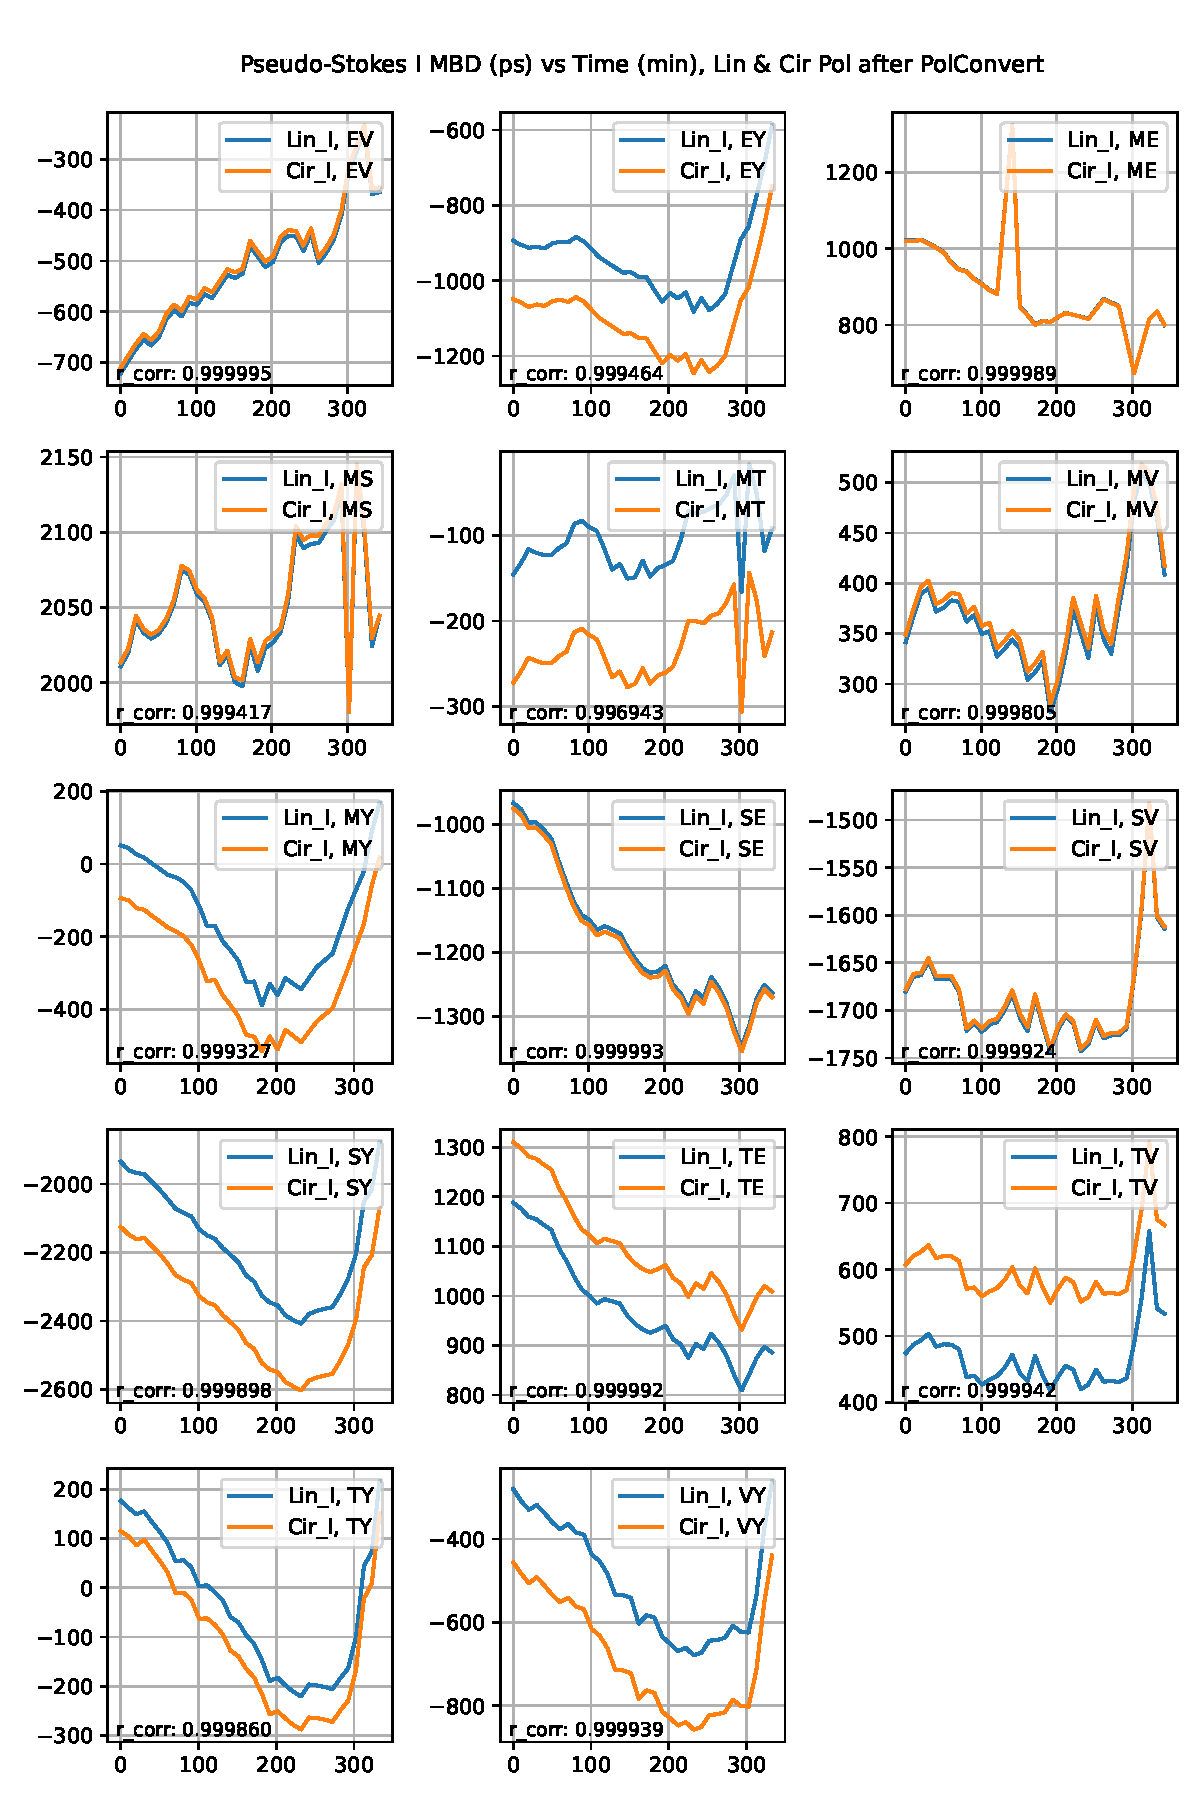
\includegraphics[width=33pc]{MBD_Lin_I_and_Cir_I.pdf}
  \caption{\small Evolution of Multi-Band Delays (in picoseconds) during the experiment (time in minutes) for the pseudo-Stokes $\protect I$ parameter for every baseline. Each panel shows two curves: LinI, $\protect I$ from the original, linearly polarized data set and CirI, $\protect I$ from the circularly polarized data set obtained by applying PolConvert to the original data. Graphs have large biases. However, the coefficients of correlation r\_corr between LinI and CirI are so close to unity that the curves can be considered identical (except for the biases).}
  \label{mbd_lin_and_cir}
  \end{center}
\end{figure}


\begin{figure}[ht!]
  \begin{center}
  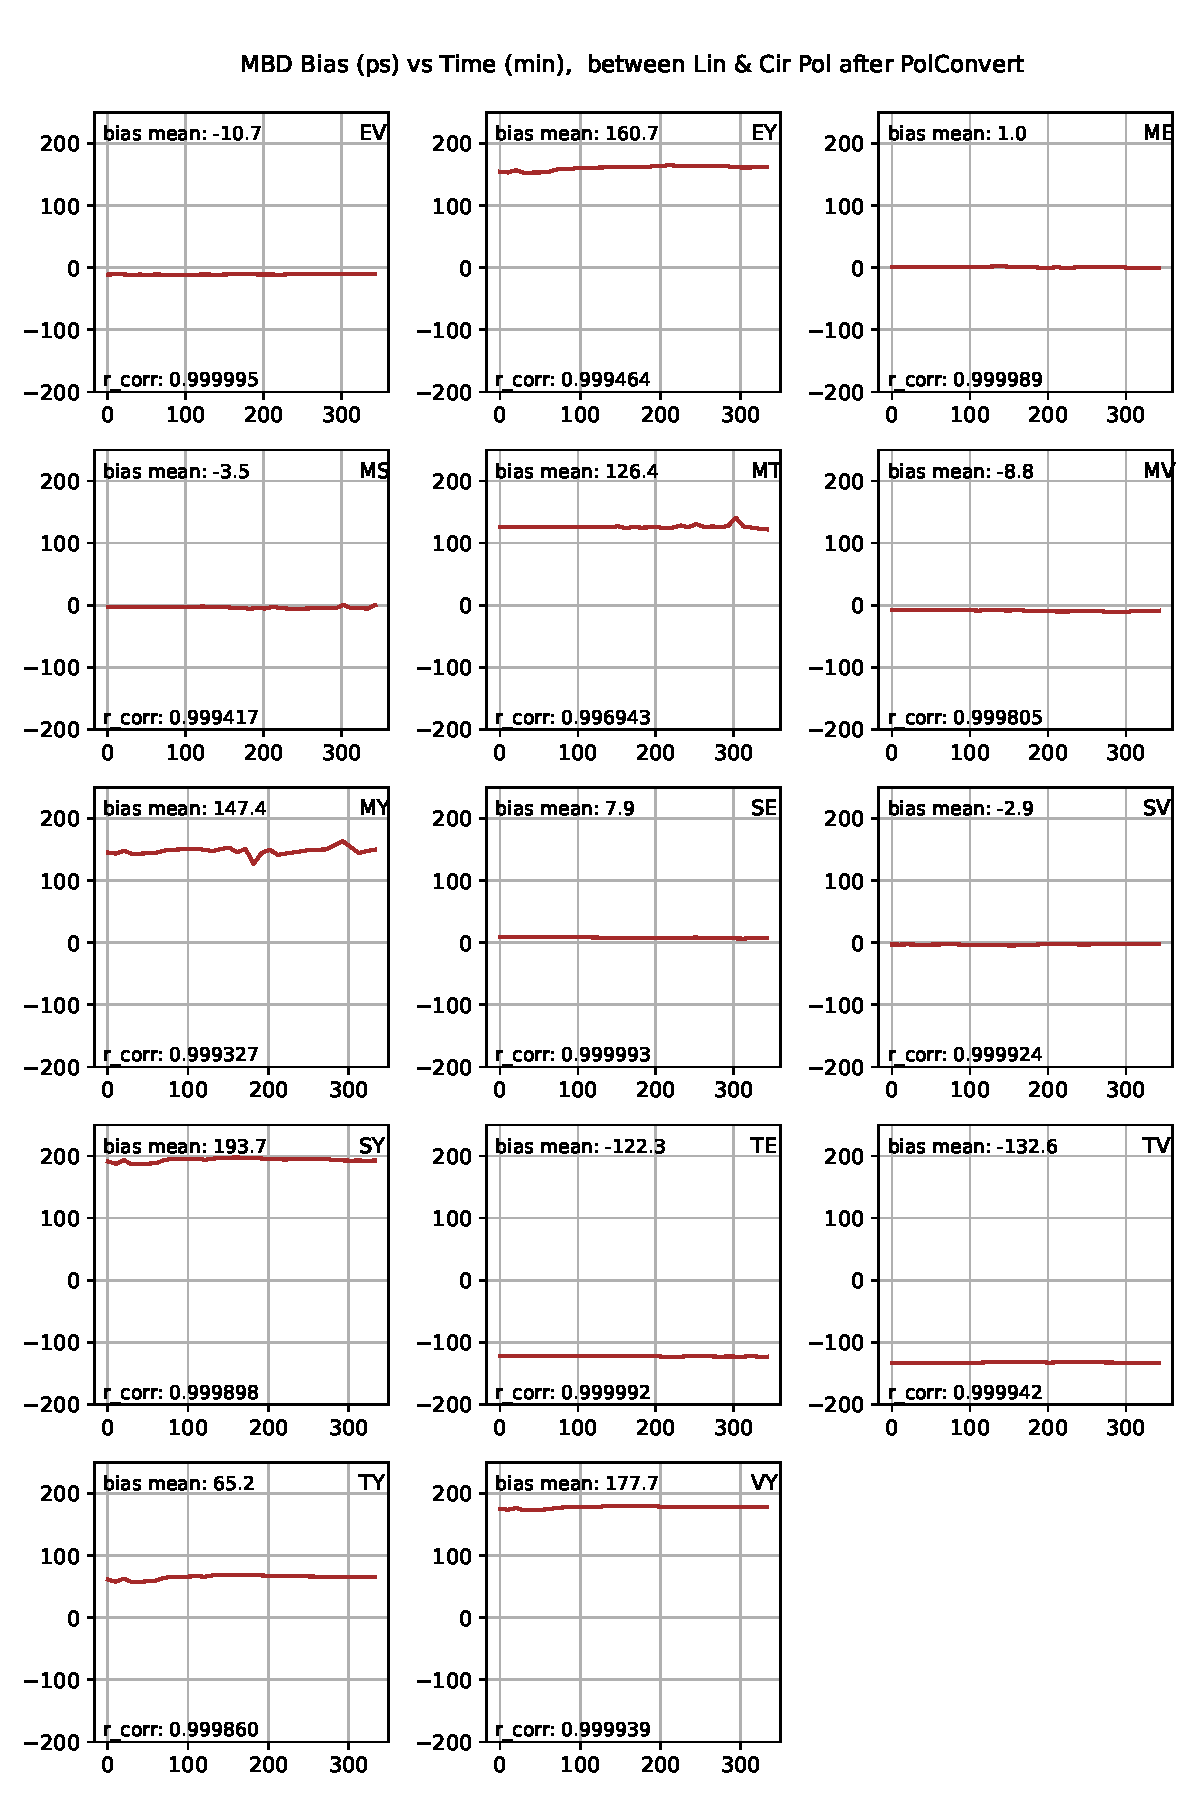
\includegraphics[width=33pc]{MBD_bias_between_Lin_I_and_Cir_I.pdf}
  \caption{\small Evolution of the bias between LinI and CirI Multi-Band Delays (in picoseconds) during the experiment (time in minutes) for the pseudo-Stokes $\protect I$ parameter for every baseline. Each panel shows one curve of LinI - CirI, where LinI is $\protect I$ from the original, linearly polarized data set and CirI is $\protect I$ from the circularly polarized data set obtained by applying PolConvert to the original data. The means for each curve and the coefficients of correlation r\_corr between LinI and CirI are given.}
  \label{mbd_lin_cir_bias}
  \end{center}
\end{figure}


\begin{figure}[ht!]
  \begin{center}
  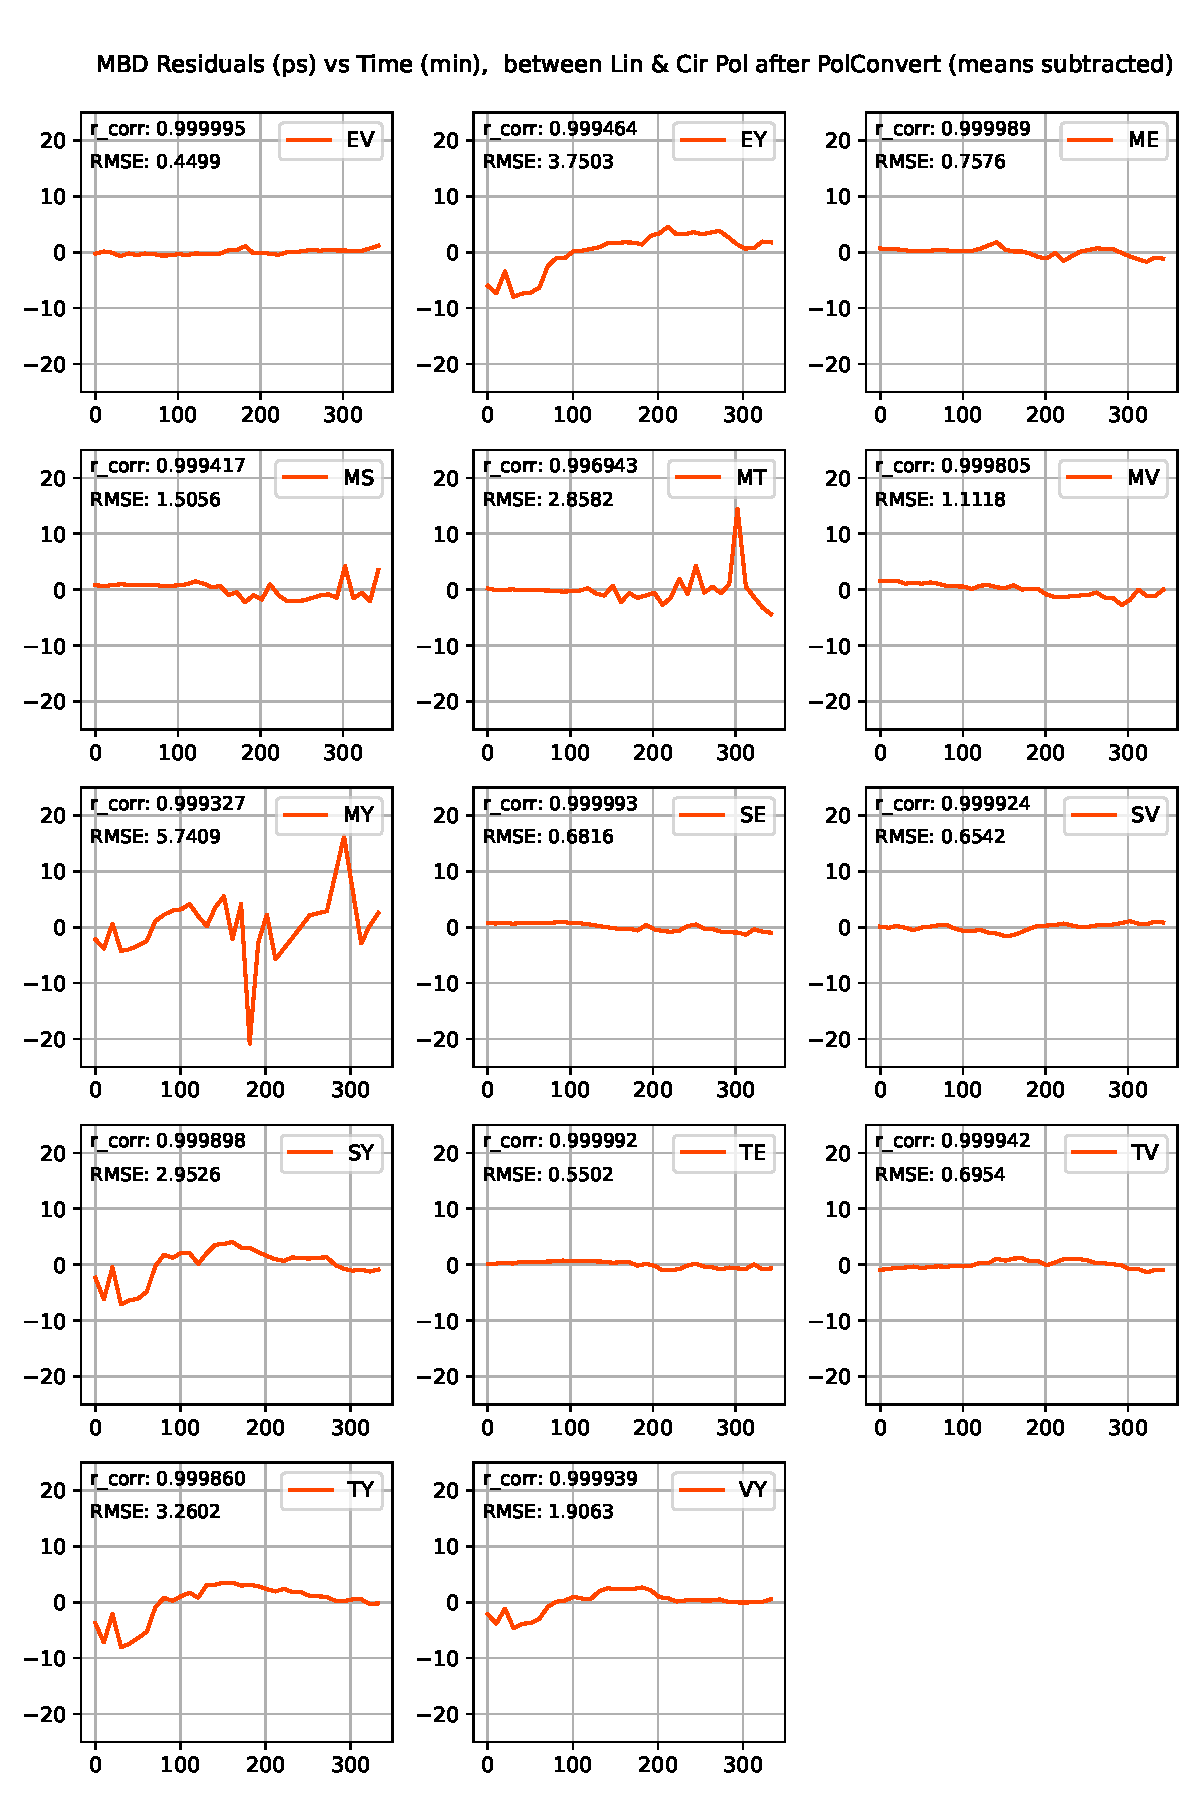
\includegraphics[width=33pc]{MBD_Lin_I_minus_Cir_I.pdf}
  \caption{\small Evolution of the residuals between unbiased LinI and CirI Multi-Band Delays (in picoseconds) during the experiment (time in minutes) for the pseudo-Stokes $\protect I$ parameter for every baseline. Each panel shows one curve of LinI - CirI, both with subtracted means, where LinI is $\protect I$ from the original, linearly polarized data set and CirI is $\protect I$ from the circularly polarized data set obtained by applying PolConvert to the original data. The coefficients of correlation r\_corr between LinI and CirI are very close to unity. The Root Mean Square Error (RMSE) shows the standard deviation of the residuals.}
  \label{mbd_lin_minus_cir}
  \end{center}
\end{figure}


\begin{figure}[ht!]
  \begin{center}
  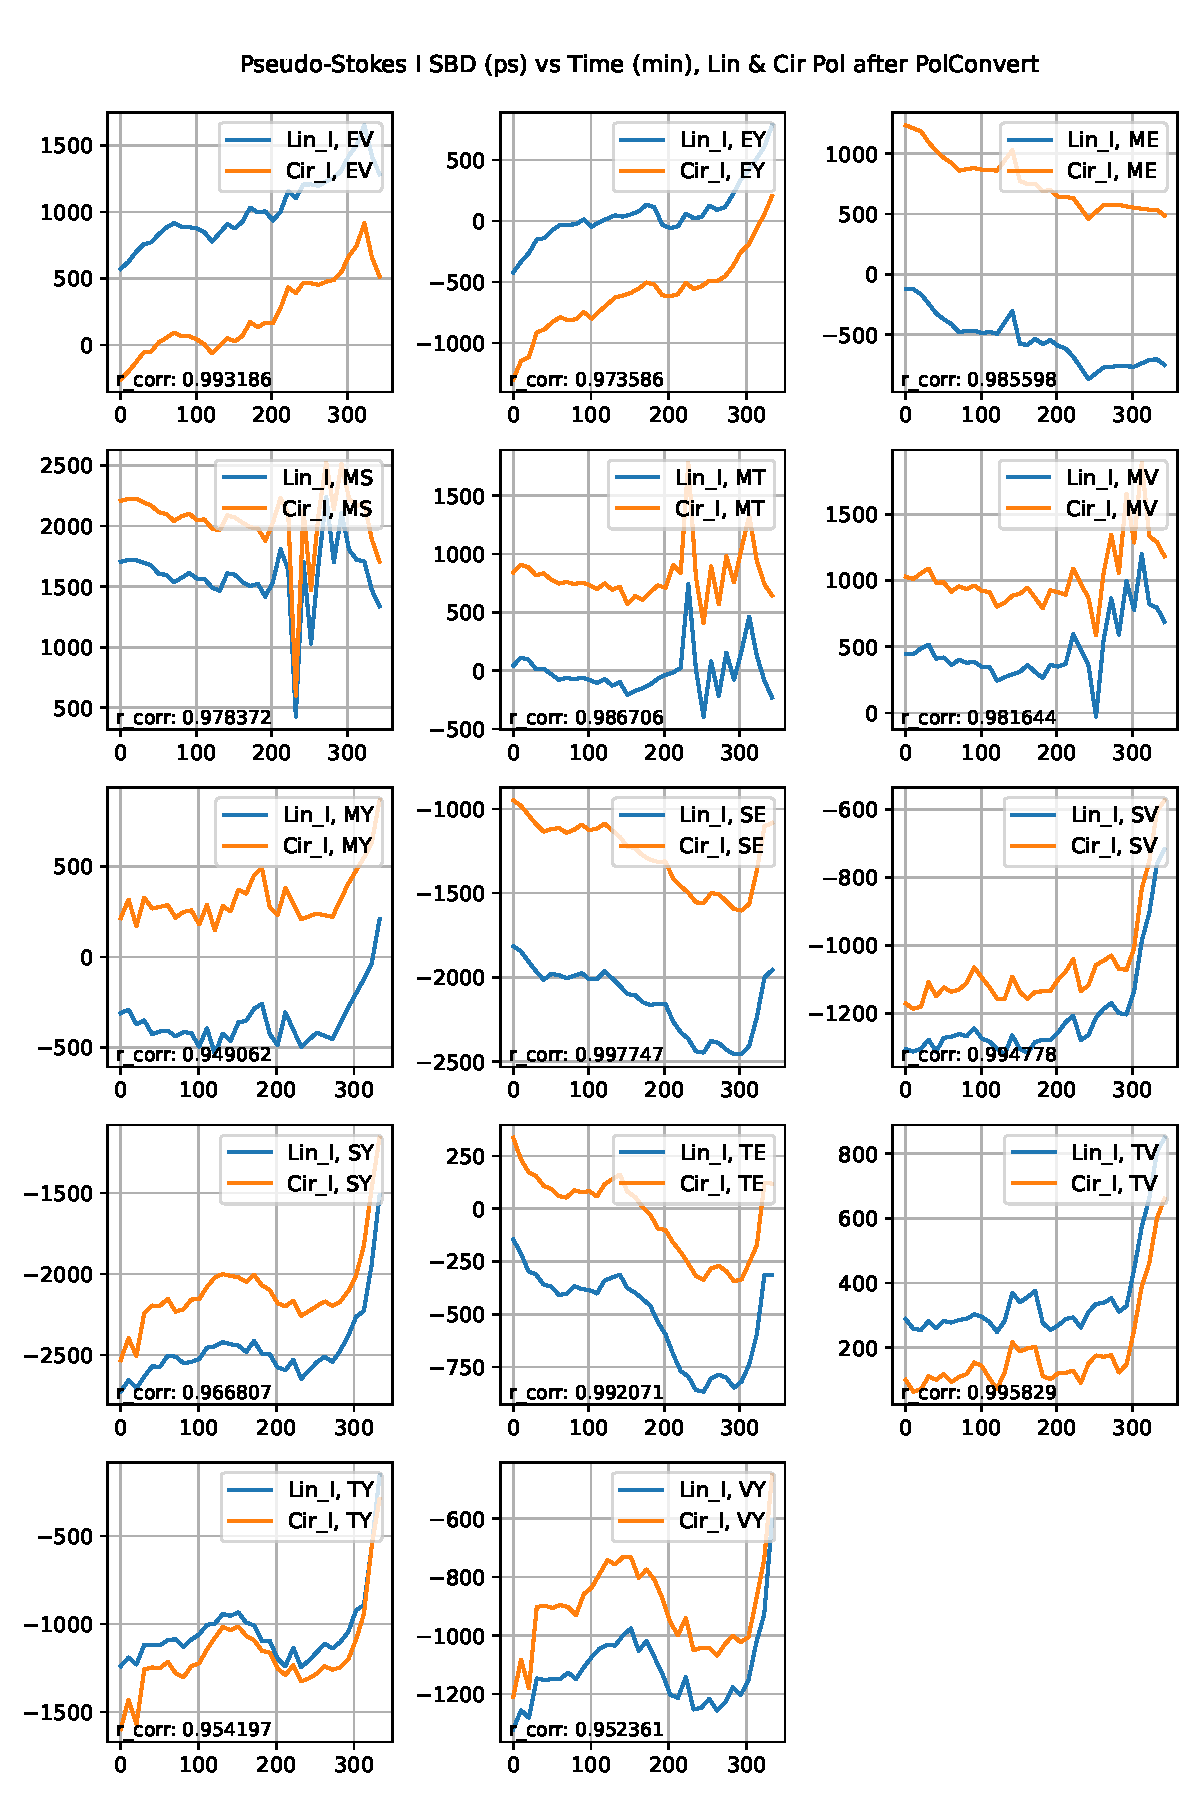
\includegraphics[width=33pc]{SBD_Lin_I_and_Cir_I.pdf}
  \caption{\small Evolution of Single-Band Delays (inpicoseconds) during the experiment (time in minutes) for the pseudo-Stokes $\protect I$ parameter for every baseline. Each panel shows two curves: LinI, $\protect I$ from the original, linearly polarized data set and CirI, $\protect I$ from the circularly polarized data set obtained by applying PolConvert to the original data. Graphs have large biases. The coefficients of correlation r\_corr between Lin\_I and CirI for most of the baselines are close to unity. If it were not for the biases, the curves could be considered close to identical.}
  \label{sbd_lin_and_cir}
  \end{center}
\end{figure}


\begin{figure}[ht!]
  \begin{center}
  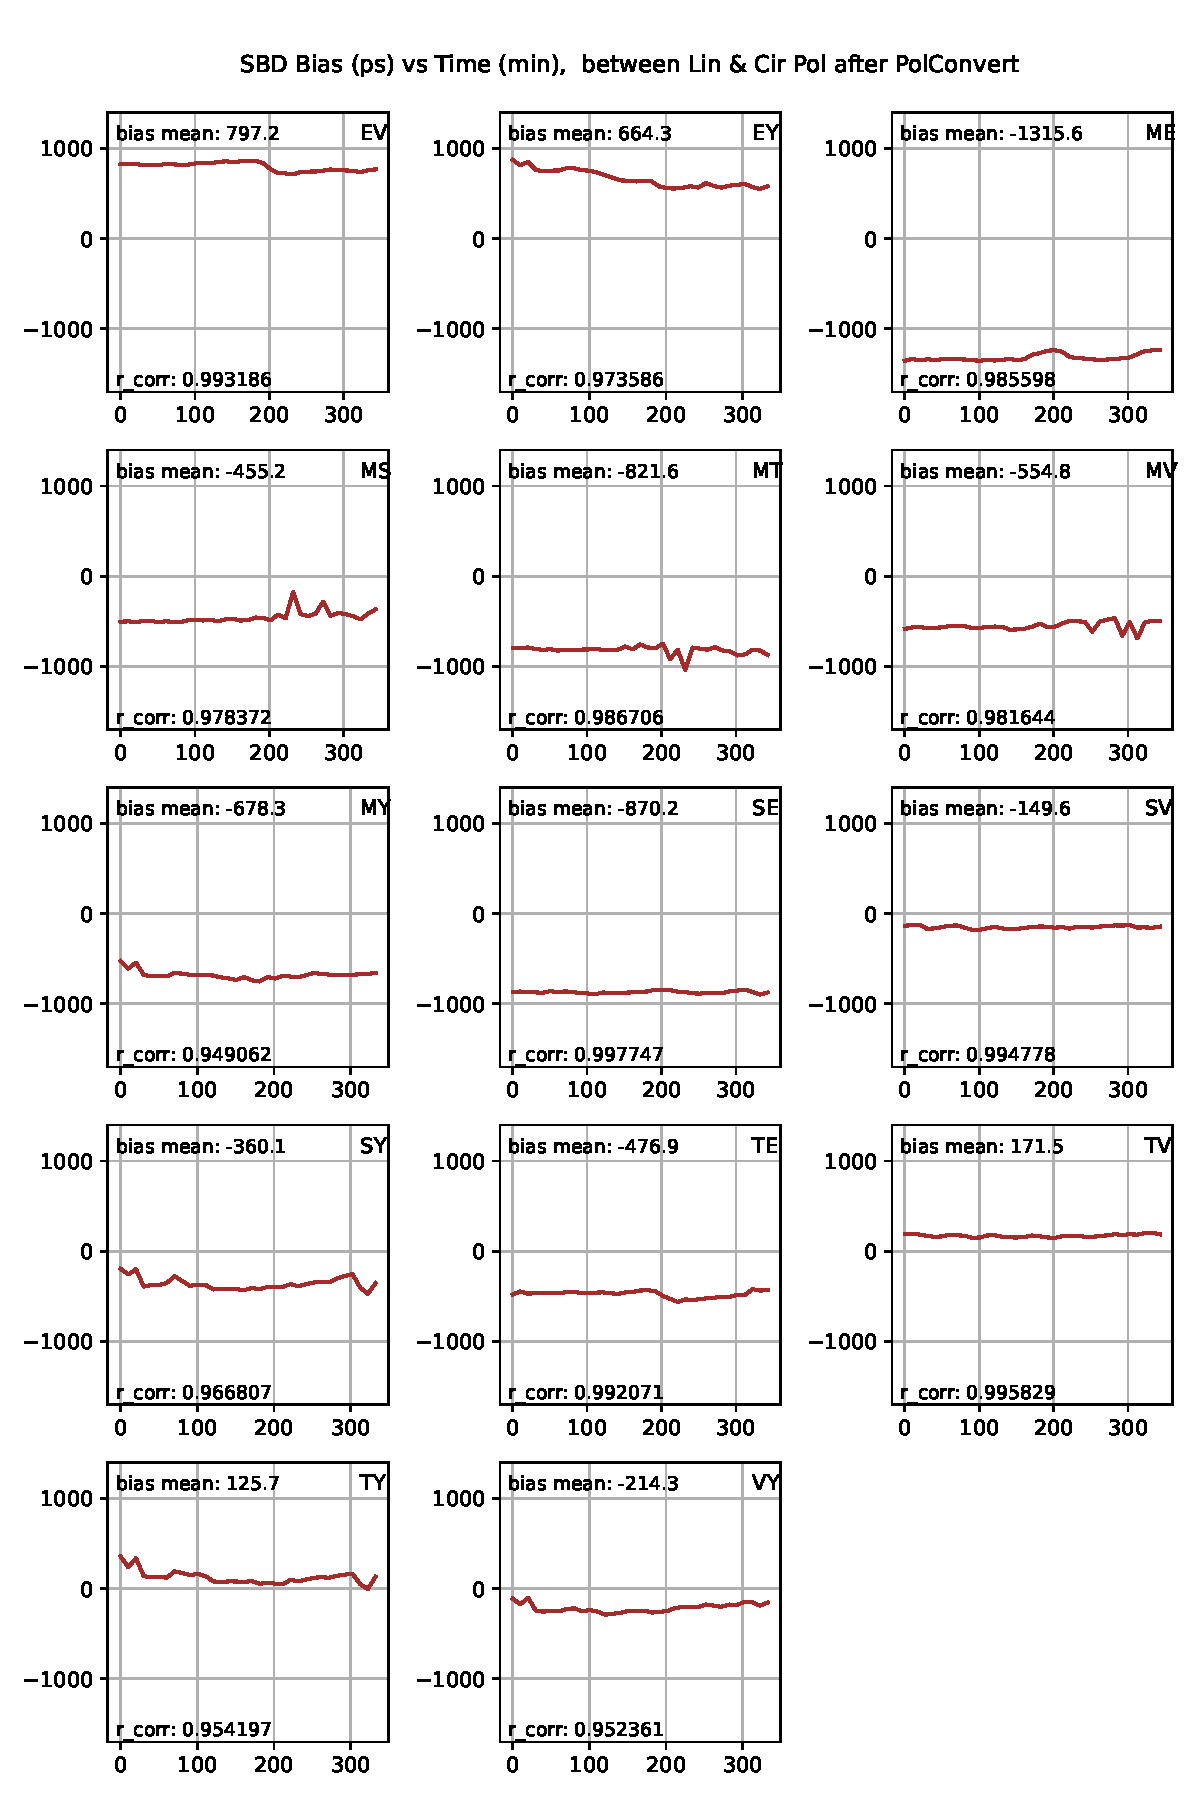
\includegraphics[width=33pc]{SBD_bias_between_Lin_I_and_Cir_I.pdf}
  \caption{\small Evolution of the bias between LinI and CirI Single-Band Delays (in picoseconds) during the experiment (time in minutes) for the pseudo-Stokes $\protect I$ parameter for every baseline. Each panel shows one curve of LinI - CirI, where LinI is $\protect I$ from the original, linearly polarized data set and CirI is $\protect I$ from the circularly polarized data set obtained by applying PolConvert to the original data. The means for each curve and the coefficients of correlation r\_corr between LinI and CirI are given.}
  \label{sbd_lin_cir_bias}
  \end{center}
\end{figure}


\begin{figure}[ht!]
  \begin{center}
  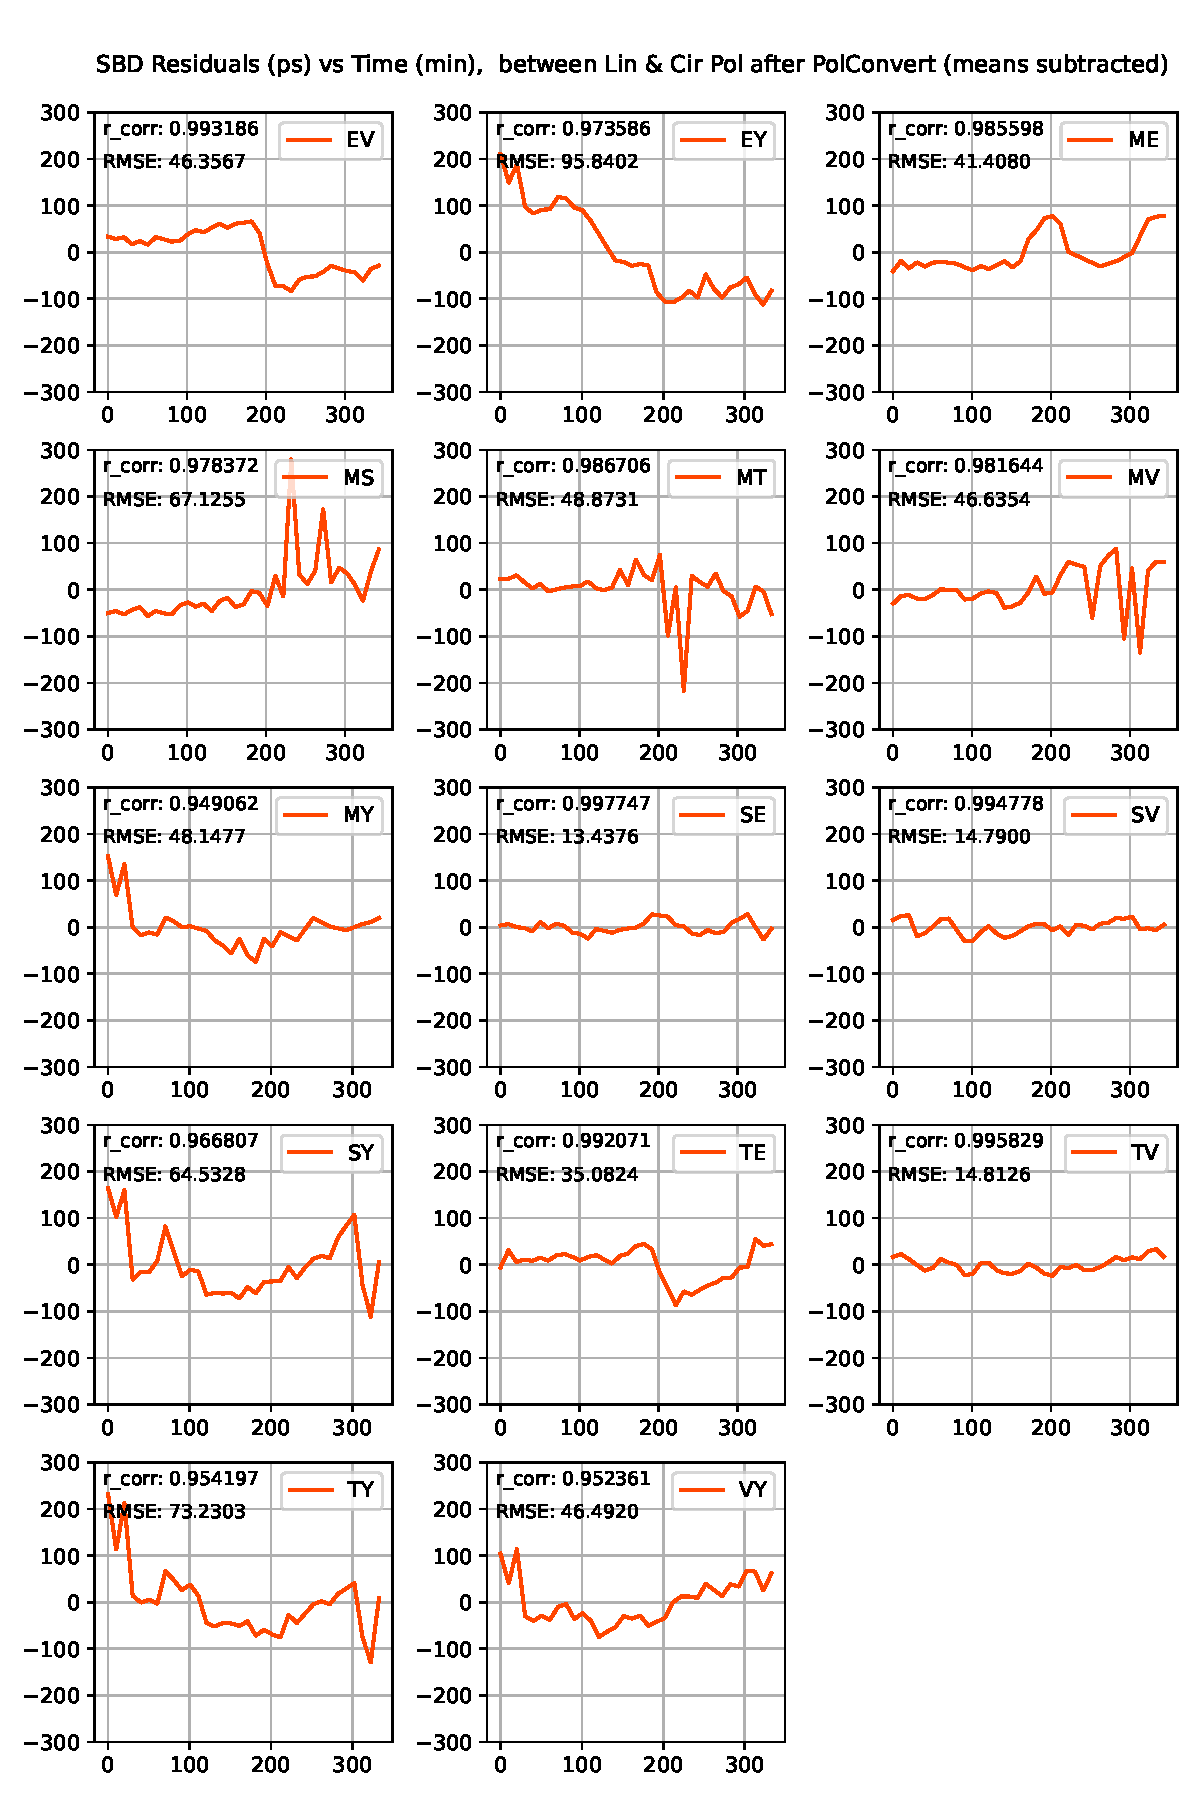
\includegraphics[width=33pc]{SBD_Lin_I_minus_Cir_I.pdf}
  \caption{\small Evolution of the residuals between unbiased LinI and CirI Single-Band Delays (in picoseconds) during the experiment (time in minutes) for the pseudo-Stokes $\protect I$ parameter for every baseline. Each panel shows one curve of LinI - CirI, both with subtracted means, where LinI is $\protect I$ from the original, linearly polarized data set and CirI is $\protect I$ from the circularly polarized data set obtained by applying PolConvert to the original data. The coefficients of correlation r\_corr between LinI and CirI are reasonably close to unity. The Root Mean Square Error (RMSE) shows the standard deviation of the residuals.}
  \label{sbd_lin_minus_cir}
  \end{center}
\end{figure}


\begin{figure}[ht!]
  \begin{center}
  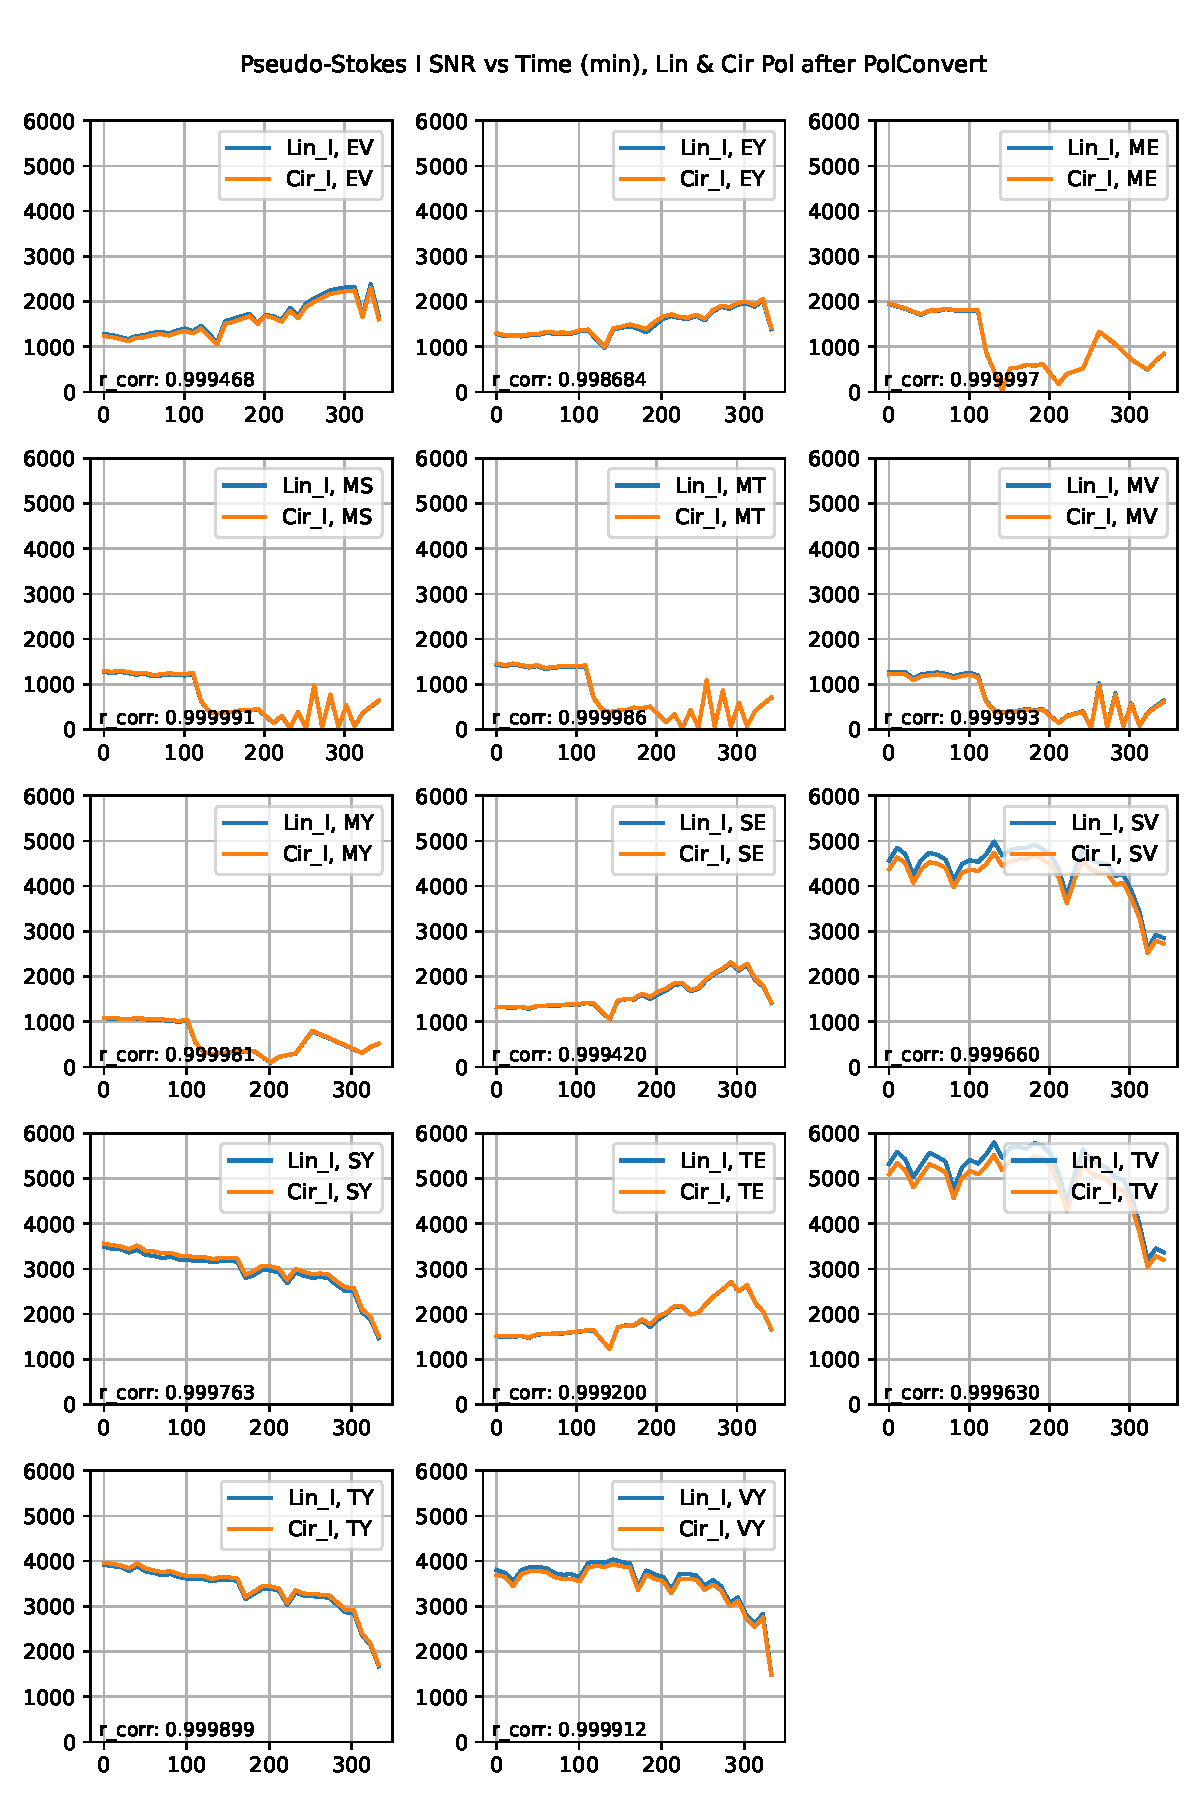
\includegraphics[width=33pc]{SNR_Lin_I_and_Cir_I.pdf}
  \caption{\small Evolution of Signal-to-Noise Ratios during the experiment (time in minutes) for the pseudo-Stokes $\protect I$ parameter for every baseline. Each panel shows two curves: LinI, $\protect I$ from the original, linearly polarized data set and CirI, $\protect I$ from the circularly polarized data set obtained by applying PolConvert to the original data. Graphs have large biases. However, the coefficients of correlation r\_corr between LinI and CirI are so close to unity that the curves can be considered identical (except for the biases).}
  \label{snr_lin_and_cir}
  \end{center}
\end{figure}



\begin{figure}[ht!]
  \begin{center}
  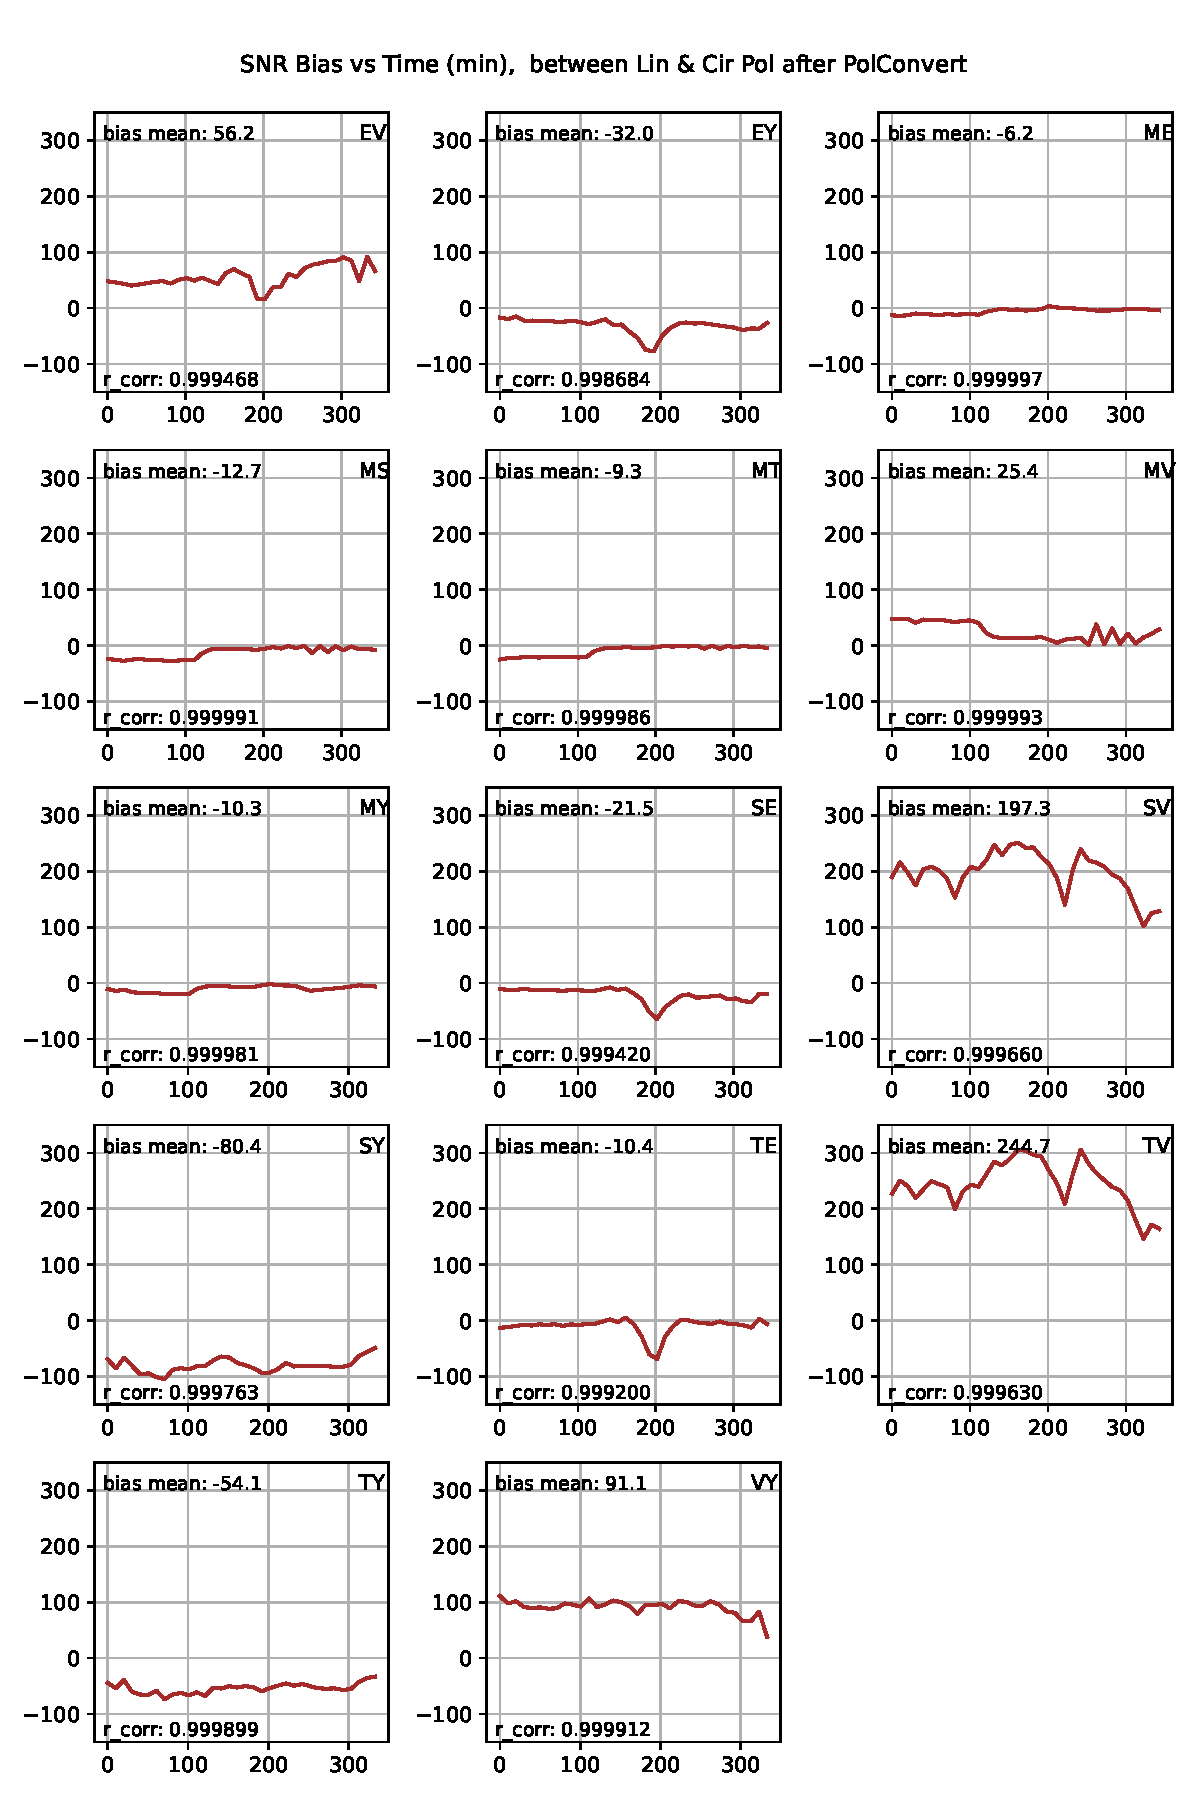
\includegraphics[width=33pc]{SNR_bias_between_Lin_I_and_Cir_I.pdf}
  \caption{\small Evolution of the bias between LinI and CirI Signal-to-Noise Ratios during the experiment (time in minutes) for the pseudo-Stokes $\protect I$ parameter for every baseline. Each panel shows one curve of LinI - CirI, where LinI is $\protect I$ from the original, linearly polarized data set and CirI is $\protect I$ from the circularly polarized data set obtained by applying PolConvert to the original data. The means for each curve and the coefficients of correlation r\_corr between LinI and CirI are given.}
  \label{snr_lin_cir_bias}
  \end{center}
\end{figure}


\begin{figure}[ht!]
  \begin{center}
  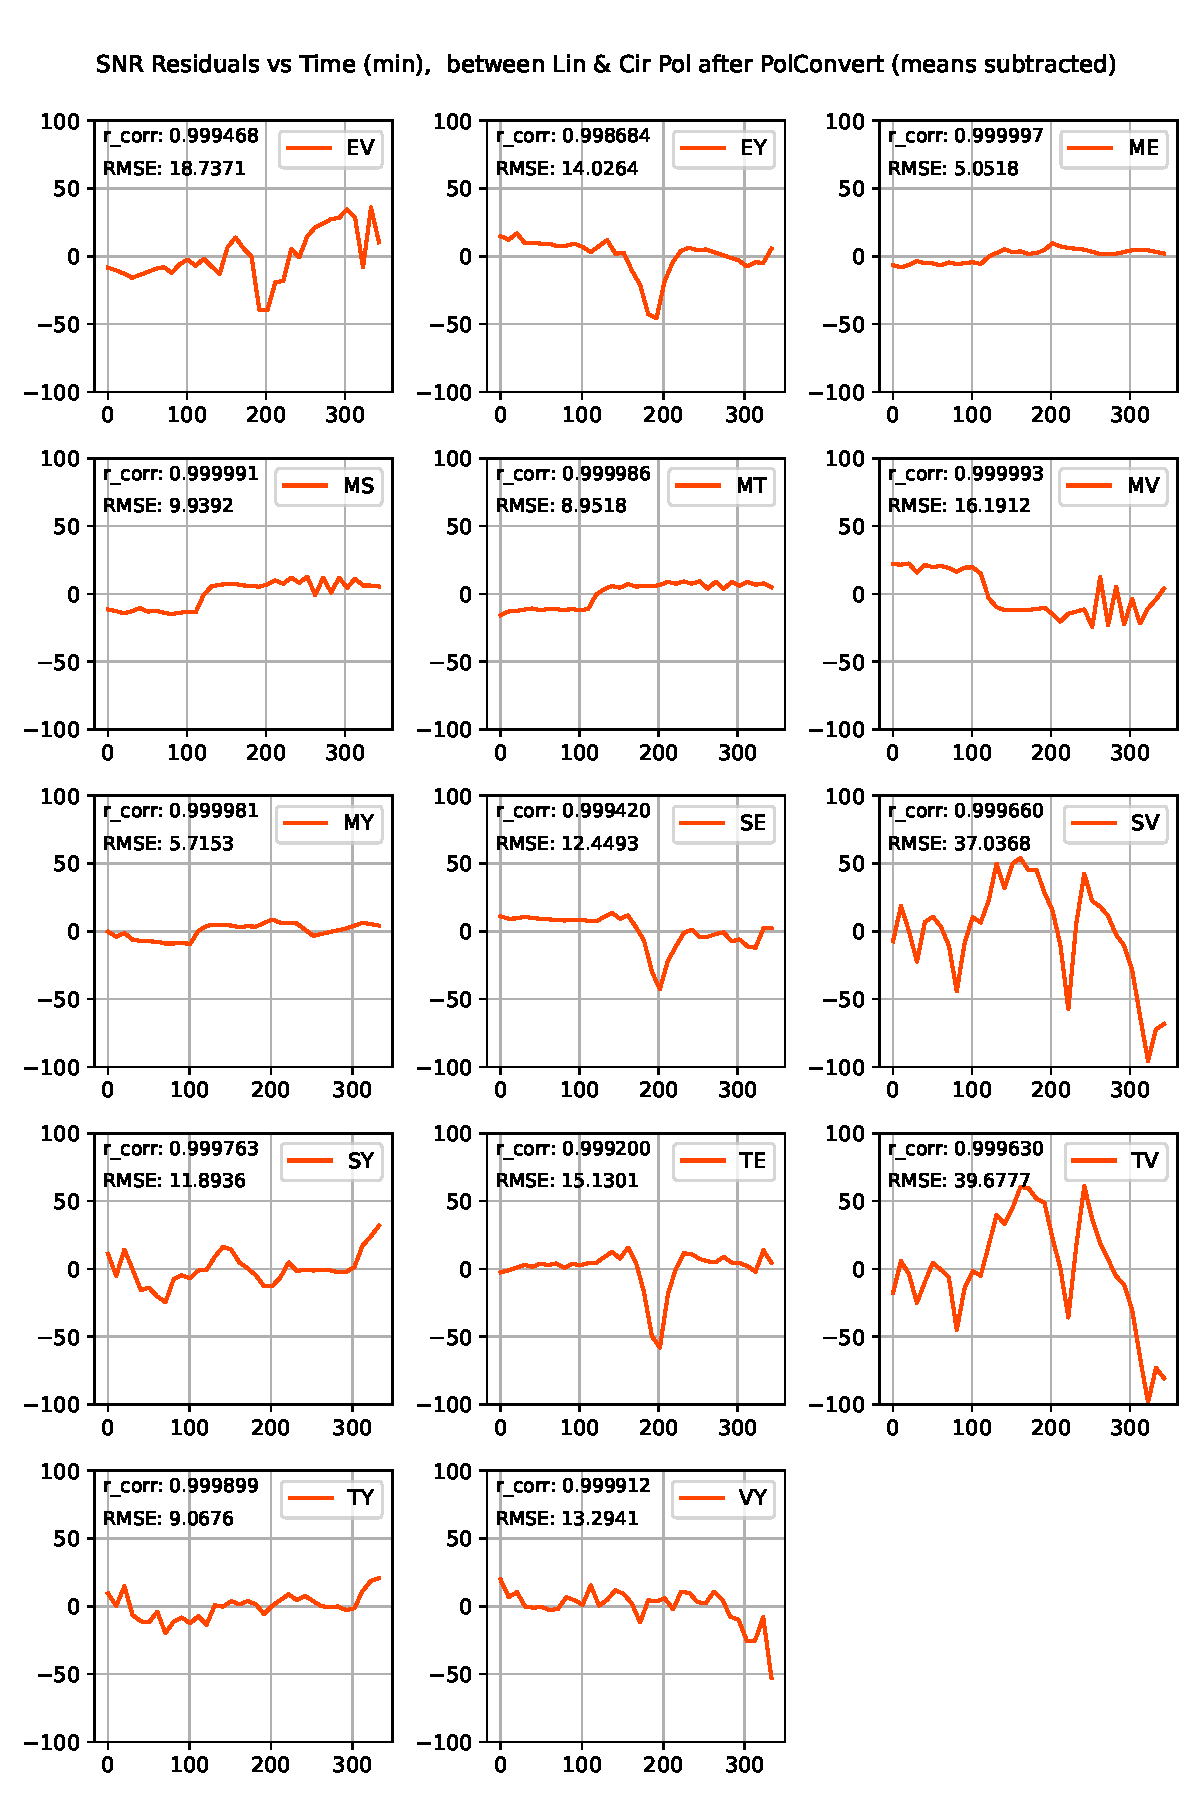
\includegraphics[width=33pc]{SNR_Lin_I_minus_Cir_I.pdf}
  \caption{\small  Evolution of the residuals between unbiased LinI and CirI Signal-to-Noise Ratios during the experiment (time in minutes) for the pseudo-Stokes $\protect I$ parameter for every baseline. Each panel shows one curve of LinI - CirI, both with subtracted means, where LinI is $\protect I$ from the original, linearly polarized data set and CirI is $\protect I$ from the circularly polarized data set obtained by applying PolConvert to the original data. The coefficients of correlation r\_corr between LinI and CirI are very close to unity. The Root Mean Square Error (RMSE) shows the standard deviation of the residuals.}
  \label{snr_lin_minus_cir}
  \end{center}
\end{figure}





\begin{figure}[ht!]
  \begin{center}
  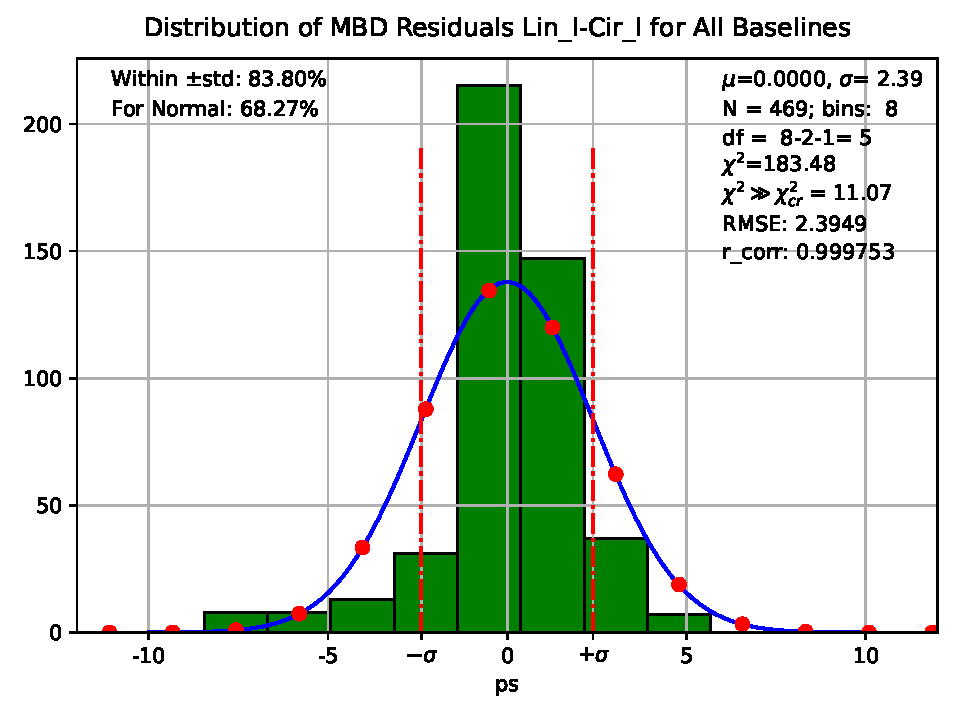
\includegraphics[width=25pc]{Distr_MBD_Lin_I-Cir_I_Diff.pdf}
  \caption{\small Histogram of the residuals (see Eq.~\eqref{resid}) for all of the baselines}
  \label{dmbd_distr}
  \end{center}
\end{figure}


\begin{figure}[ht!]
  \begin{center}
  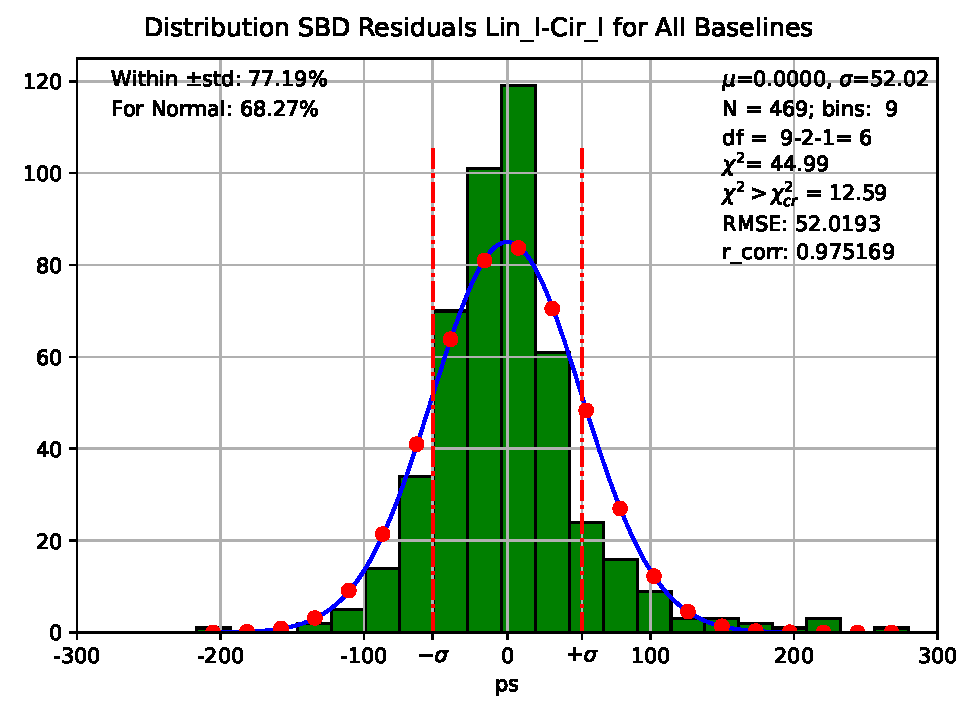
\includegraphics[width=25pc]{Distr_SBD_Lin_I-Cir_I_Diff.pdf}
  \caption{\small }
  \label{dsbd_distr}
  \end{center}
\end{figure}


\begin{figure}[ht!]
  \begin{center}
  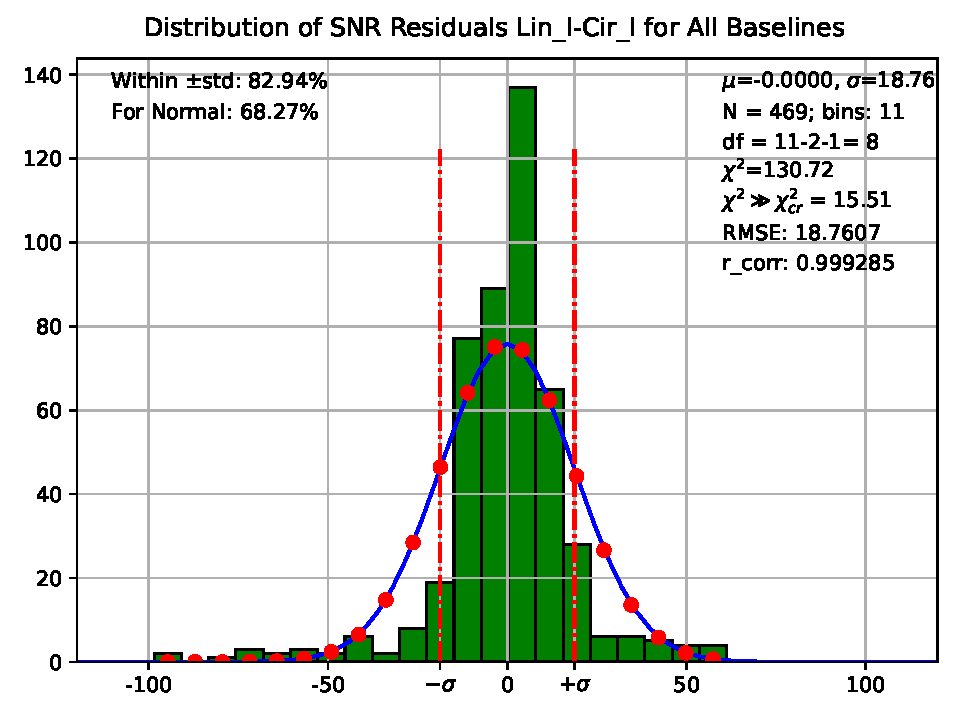
\includegraphics[width=25pc]{Distr_SNR_Lin_I-Cir_I_Diff.pdf}
  \caption{\small }
  \label{dsnr_distr}
  \end{center}
\end{figure}



\begin{figure}[ht!]
  \begin{center}
  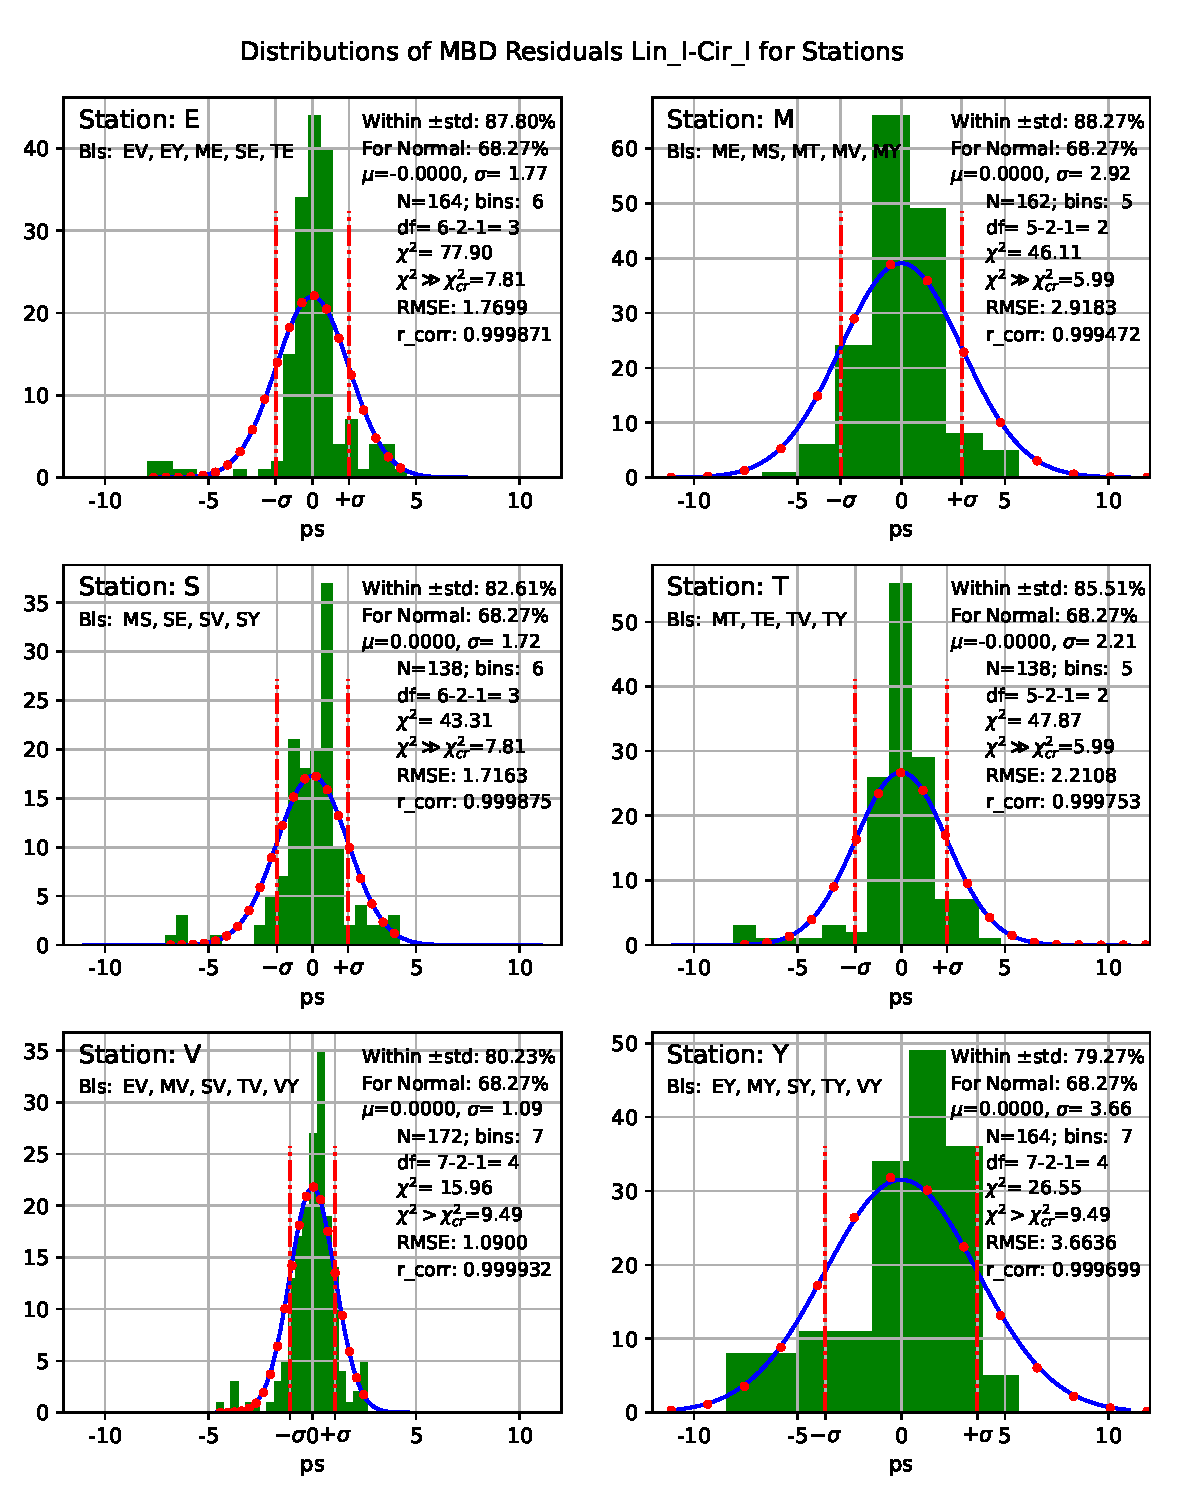
\includegraphics[width=33pc]{Distr_MBD_Lin_I-Cir_I_Diff_Stations.pdf}
  \caption{\small }
  \label{dmbd_distr_st}
  \end{center}
\end{figure}


\begin{figure}[ht!]
  \begin{center}
  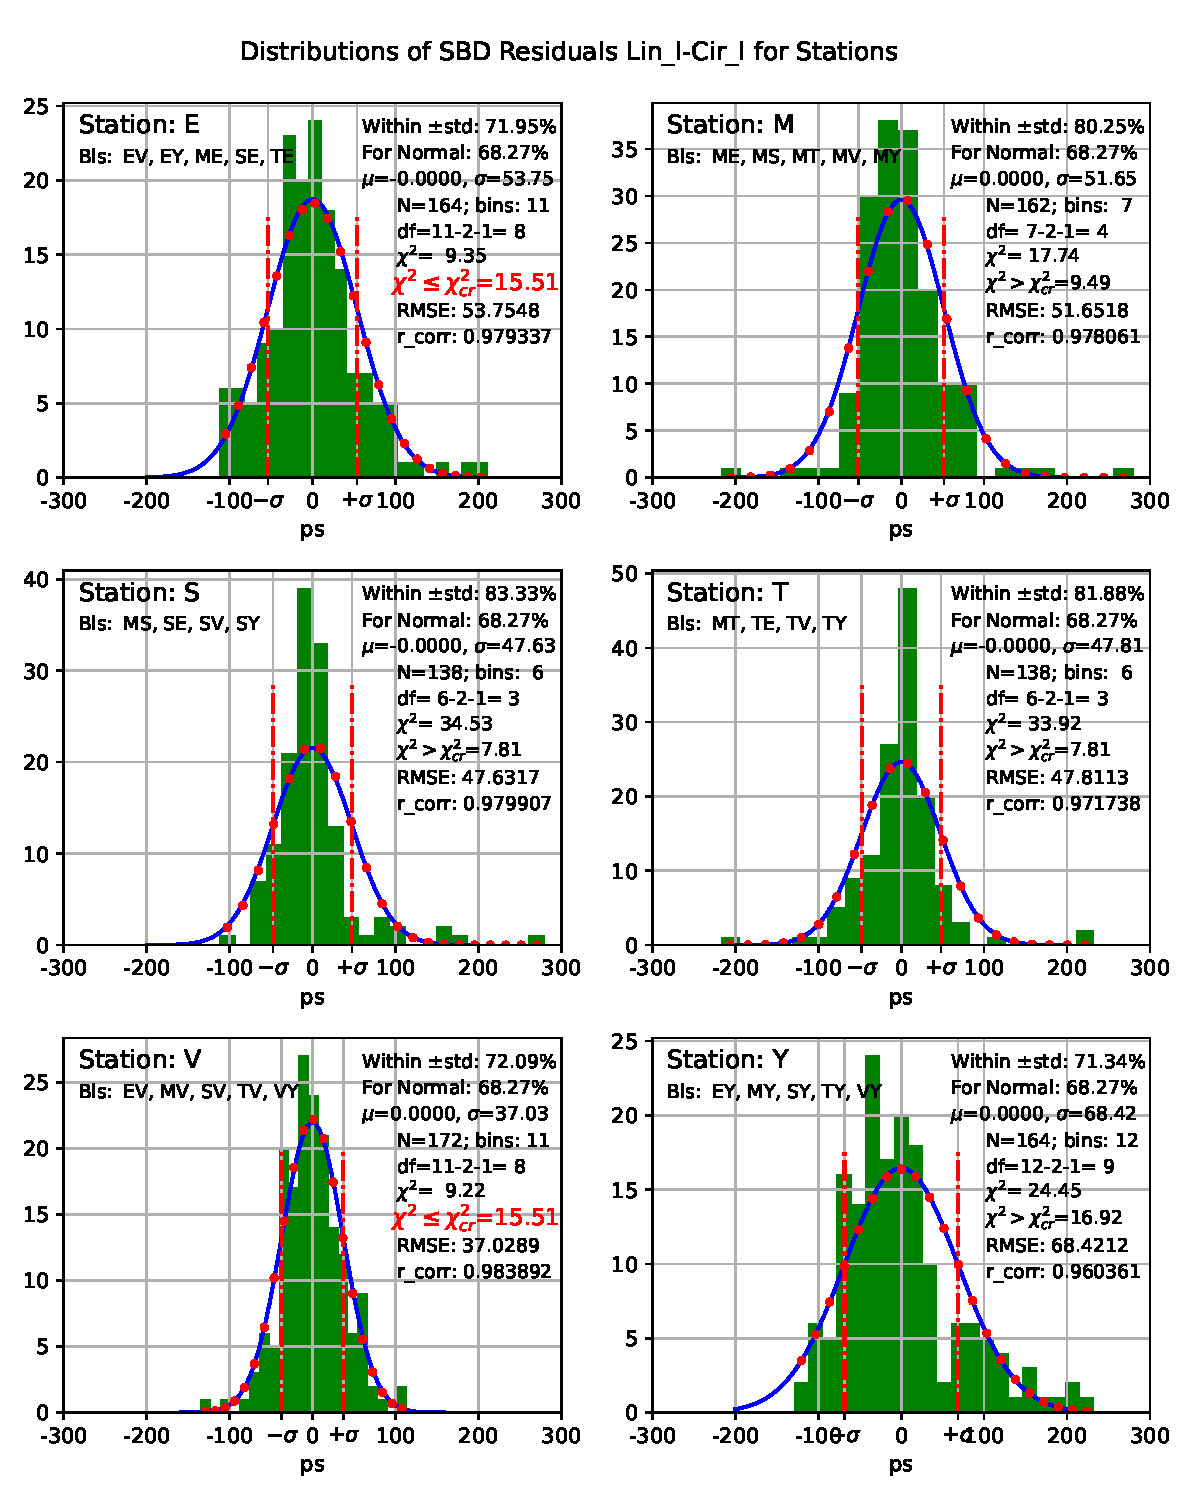
\includegraphics[width=33pc]{Distr_SBD_Lin_I-Cir_I_Diff_Stations.pdf}
  \caption{\small }
  \label{dsbd_distr_st}
  \end{center}
\end{figure}


\begin{figure}[ht!]
  \begin{center}
  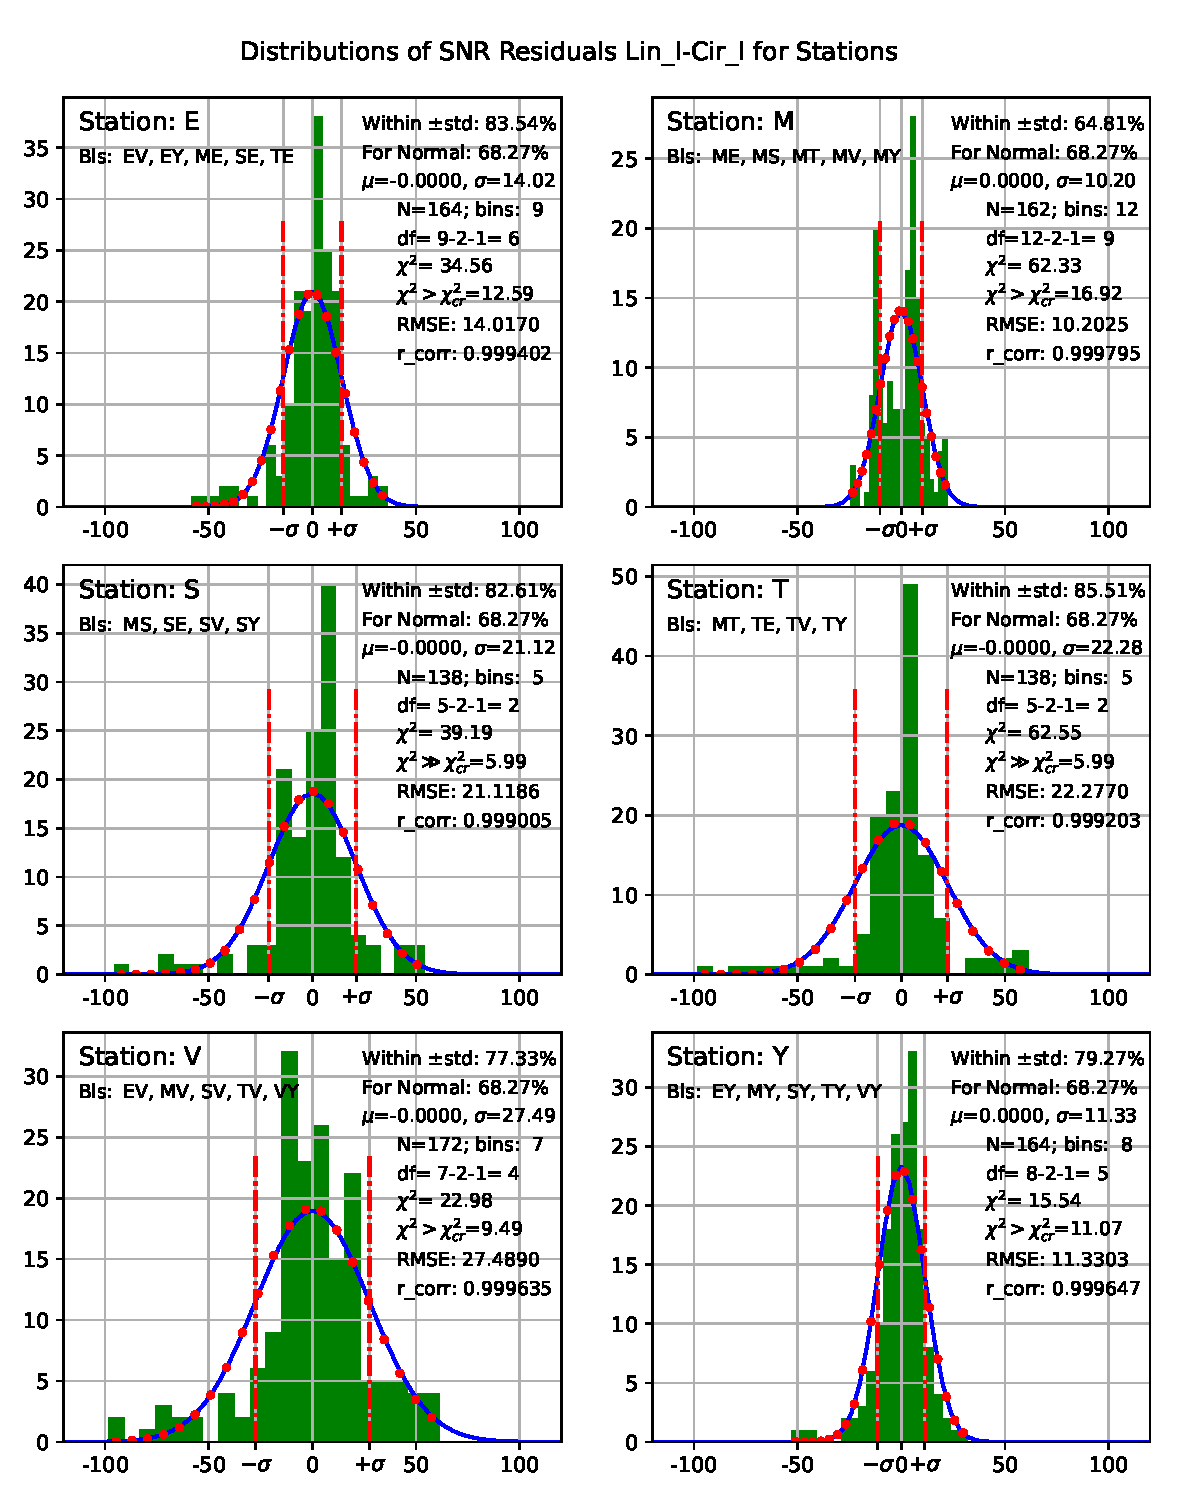
\includegraphics[width=33pc]{Distr_SNR_Lin_I-Cir_I_Diff_Stations.pdf}
  \caption{\small }
  \label{dsnr_distr_st}
  \end{center}
\end{figure}




\end{document}



